%%%%%%%%%%%%%%%%%%%%%%%%%%%%%%%%%%%%%%%%%%%%%%%%%%%%%%%%%%%%%%%%%%%%%%%
%%%                           System Description
%%%%%%%%%%%%%%%%%%%%%%%%%%%%%%%%%%%%%%%%%%%%%%%%%%%%%%%%%%%%%%%%%%%%%%





\chapter{System Description}

This chapter will discuss our game design, the story, mechanics, and tools used, and briefly discuss the previous iteration.

\section{Game Description}
The game is developed on React\footnote{https://reactjs.org/} with Chakra UI\footnote{https://chakra-ui.com}. We use Supabase\footnote{https://supabase.com/} to keep logs of user interaction with the game. Figure \ref{fig:screenshot} shows the initial state of the game.

\begin{figure}[h]
    \centering
    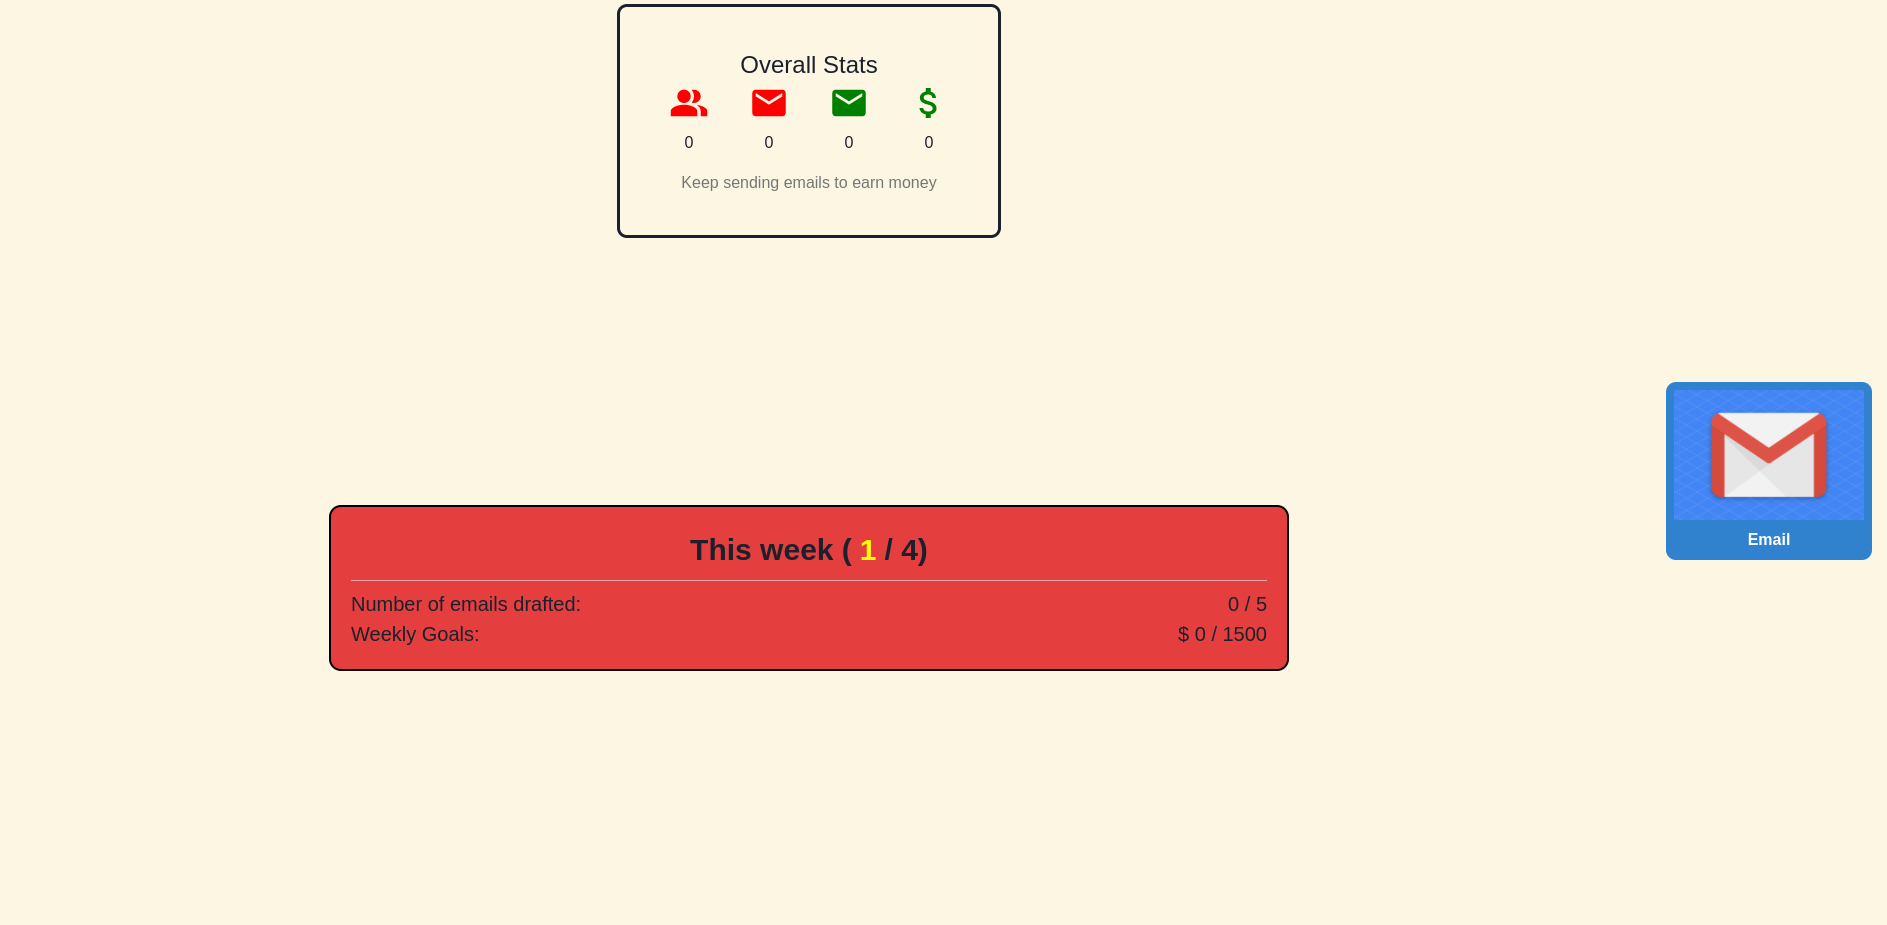
\includegraphics[width=\textwidth]{figures/section2/game.png}
    \caption{Screenshot of initial state of the game}
    \label{fig:screenshot}
\end{figure}

\subsection{Game Story}
The game's main character has taken a large loan from a loan shark. The goal of the game is to pay off the loan in time. However, as the loan is substantial, he cannot earn enough money through hard work and uses phishing tricks to scam people. The main character hires a helper to create phishing emails. The emails generated by the helper impersonate PayPal. The player has four weeks to pay off the loan with weekly payments.

\section{Mechanics}
One of our main objectives while developing the game was to streamline the player experience. We divided the game into four weeks (parts) to achieve this goal. Each week's progression will unlock specific skills users' can use to create email. We will talk more about certain week progression in later sections. Players can use the unlocked skills to generate emails. Each email efficiency will be based on the option chosen by the user.

\subsection{Components}
Before we deep dive into the flow of the game, let us talk about each individual component.

\subsubsection{Atttacker}
The attacker module takes care of training the helper. There are six different skills that the player can train the helper on, namely spelling, grammar, styling, links, spoofing, and research. We divide these skills as language skills (spelling and grammar) and technical skills (styling, links, spoofing, research). Language skills are passive skills in the game, whereas technical skills, except for styling, are active skills.

Training on passive skills will improve the quality of the email generated by the system without any additional input from the user. In contrast, active skills will give the user more options while generating the email. For example, after you train you helper on spellings, the attacker will stop making spelling errors without any additional input from the user. However, training the helper on links will allow the user to choose how to hide the links while creating the email. Table \ref{table:attacker} lists the skills and their effect in the game in brief. We will talk about the different properties activated by each skill while talking about email generation.

\begin{table}[h]
    \centering
    \begin{tabular}{p{0.05\textwidth} p{0.05\textwidth}  p{0.05\textwidth}  p{0.5\textwidth}}
        \hline
        \textbf{Skills} & \textbf{Active/} & \textbf{Cost} & \textbf{Effect}                                                   \\
                        & \textbf{Passive} &               &                                                                   \\
        \hline
        Spelling        & Passive          & 1,000         & Creates emails without spelling errors                            \\
        Grammar         & Passive          & 1,000         & Create emails without grammar errors                              \\
        Styling         & Passive          & 2,000         & Create stylized emails with better header, footer, and images     \\
        Links           & Active           & 3,000         & Unlocks different techniques to hide the link while sending email \\
        Research        & Active           & 3,000         & Gives the user option to generated targeted emails                \\
        Spoofing        & Active           & 4,000         & Gives the user ability to spoof the email                         \\
        \hline
    \end{tabular}
    \caption{Different skills and their effect in the game}
    \label{table:attacker}
\end{table}

We chose the skills in the game to replicate the training objective of existing training modules and common properties found in phishing emails. Each skill in the game has a training cost associated with it. Skills were not made free to represent training requires some resources. However, the cost is kept at a minimum to let the user unlock it as soon as possible but scaled such that more efficient skills have a higher price than general skills. Keeping the cost low allowed the user to focus more on using those skills to generate emails rather than earning money to train attackers.

Although we tried to include all the common properties found in phishing emails, we could not itemize some general properties such as sense of urgency, generic greetings, too good to be true emails, etc. Therefore, the decision to limit the number of skills was primarily made to limit the number of properties users were actively concentrating on. On the technical side, the limited number of properties to look at while generating emails made email generation much more manageable and allowed us to generate a wide range of emails. Emails generated by the system still include these properties.

% We believe although the we didnt include these in active gameplay, there are some passive gameplay that will trigger the user instinct.
\begin{figure}[ht]
    \centering
    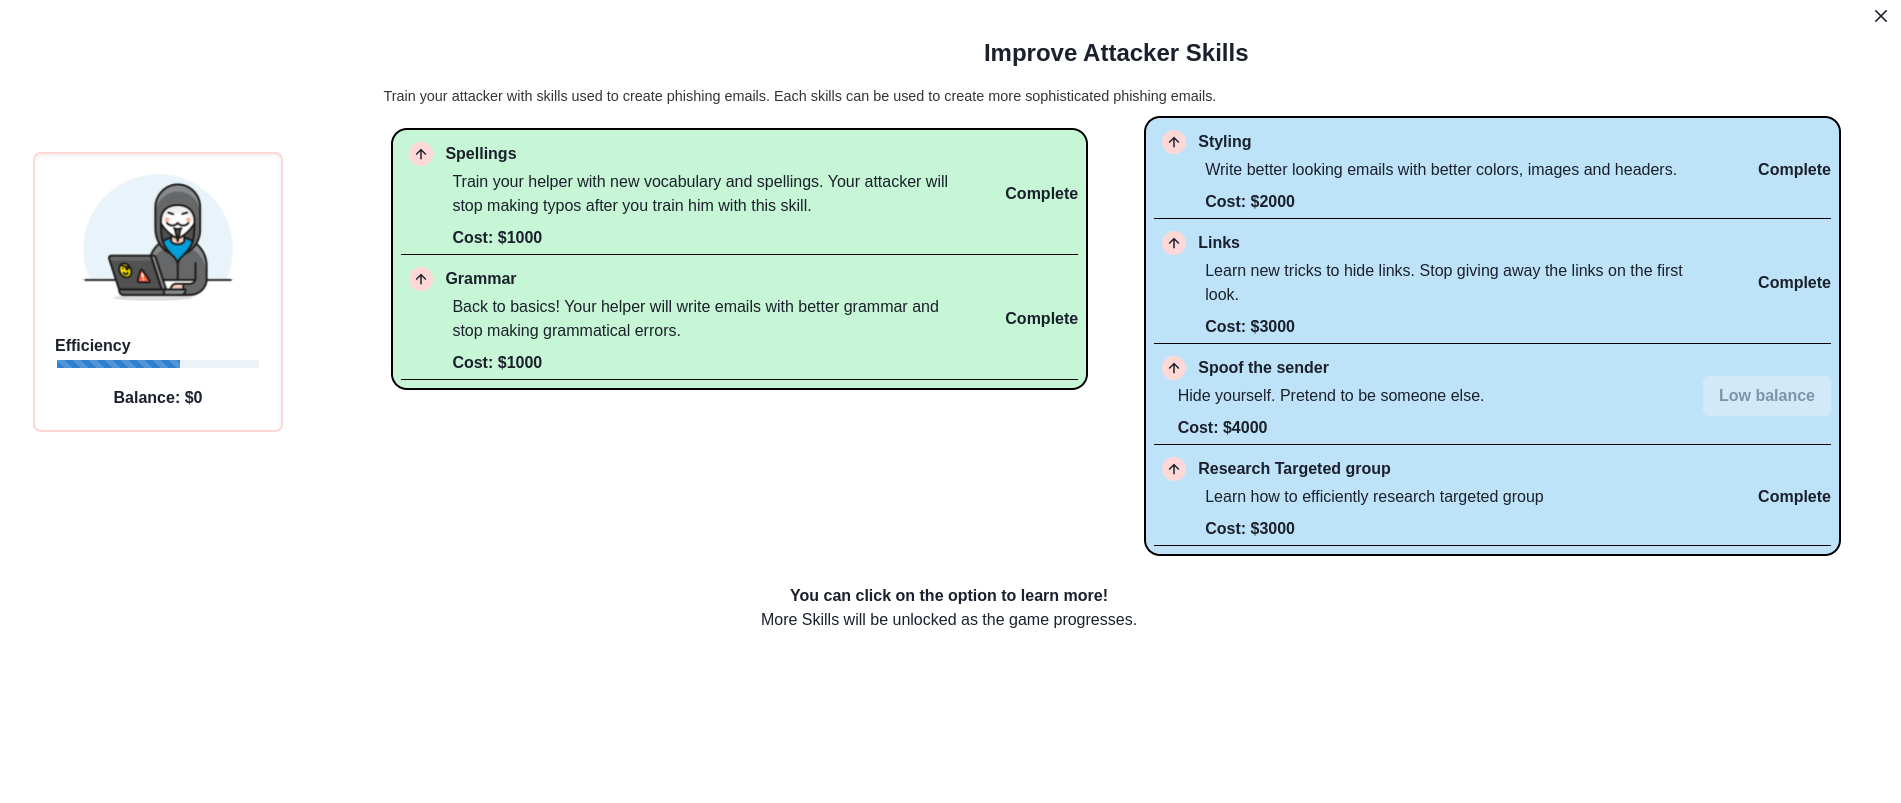
\includegraphics[width=1.1\textwidth]{figures/section2/attacker.png}
    \caption{Screenshot of the attacker module on week 4}
    \label{fig:attacker}
\end{figure}

\subsubsection{Marketplace}
The marketplace allows the player to purchase domains that can be used while generating emails (See figure \ref{fig:marketplace}). Existing training modules train the players to recognize phishing links (which are generated by the system) but do not allow players to try custom domains. In our gameplay, the attacker "Link" skill teaches how phishing emails hide links to trick victims into clicking the link.

\begin{figure}
    \centering
    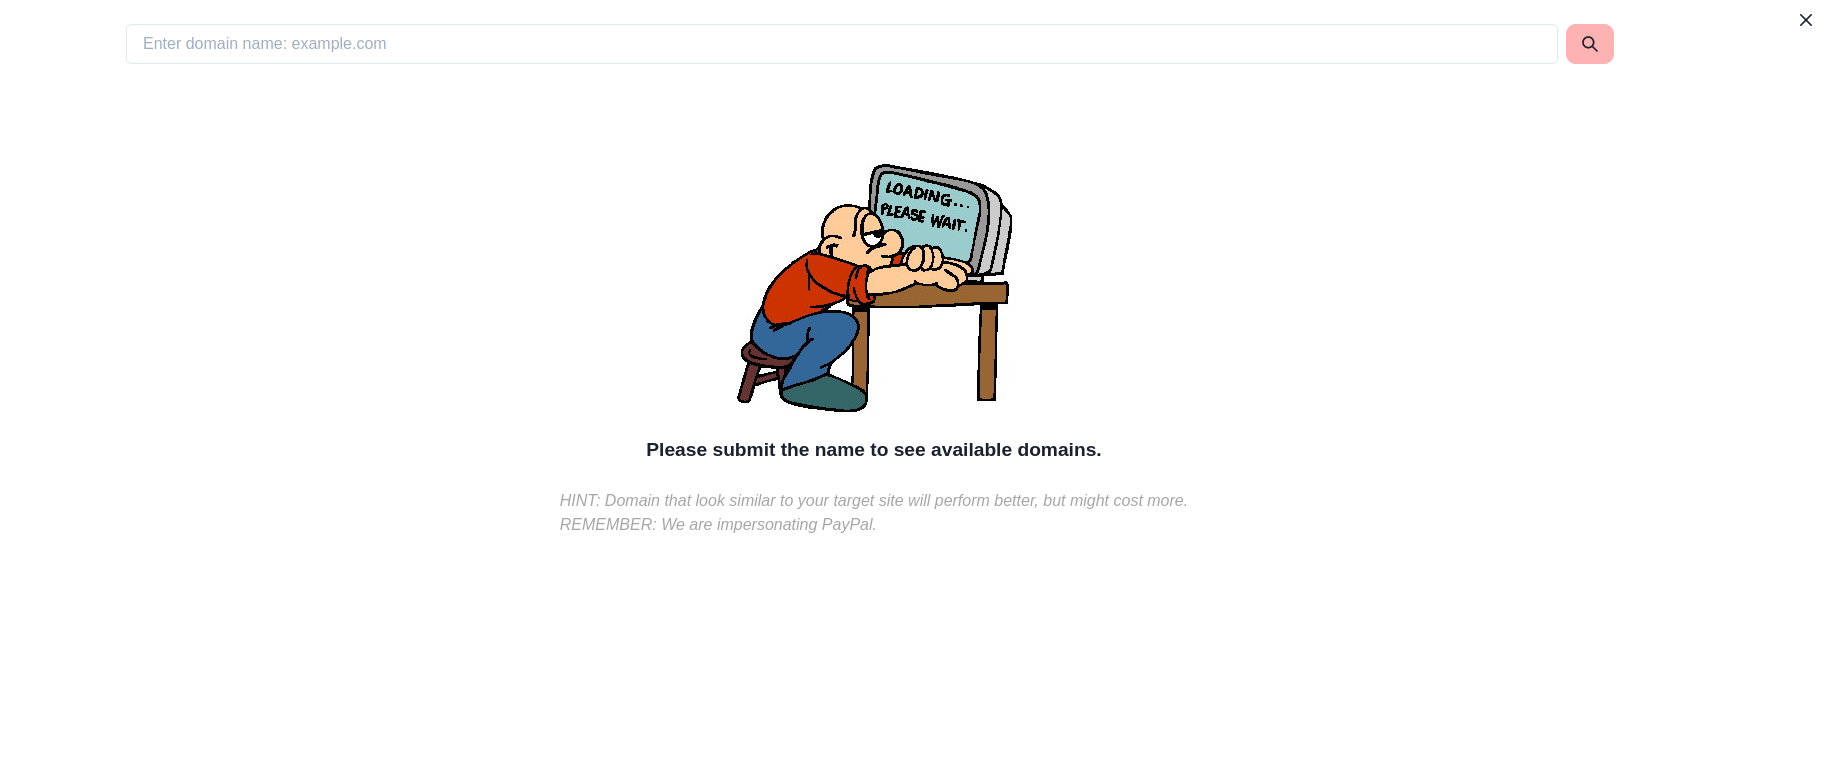
\includegraphics[width=1\textwidth]{figures/section2/marketplace_empty.png}
    \caption{The marketplace accepts any valid domain name}
    \label{fig:marketplace}
\end{figure}

The first step when letting the user purchase a domain is to check if the domain is valid. A valid domain is a second-level domain followed by a top-level domain in our game. For example, "test.com" is a valid domain where "test" is a second-level domain and "com" is the top-level domain. The validity of the second-level domain is based on the characters in the domain. We do not allow special characters (Fada Accent) in our domain for simplicity. The following regex code validates the domain:

\begin{lstlisting}
    if (userLink.includes(" ") || !/^[a-zA-Z0-9-.]*$/.test(userLink))
        return;
\end{lstlisting}

There are 1,500 top-level domain \cite{tld}. We only allow users to choose from a predefined list filtered from Tranco list \cite{trancos}. Tranco list provides us with the most popular one million domains. We filtered 262 top-level domains from the Tranco list that occur at least one hundred times. This limited number of top-level domains allowed us to incorporate commonly used domains while maintaining the game's simplicity.

\begin{figure}[h]
    \centering
    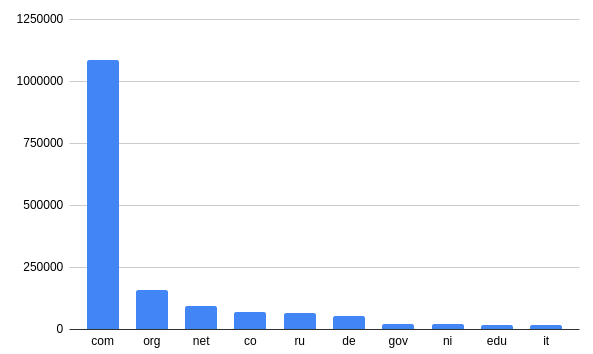
\includegraphics[width=0.5\textwidth]{figures/section2/tld.png}
    \caption{Top 10 top level domains present Tranco list}
    \label{fig:marketplace_tld}
\end{figure}

Players can choose any combination of valid characters for the second-level domain (validated by the regex pattern shown above). For example, "123test.com" is a valid domain. However, "\%ssda1.com" is not a valid domain. We maintain the top 1000 domains in the Tranco list to prevent purchasing popular and already existing domains. This list consists of popular sites such as "google.com," "facebook.com," "netflix.com," including "paypal.com" (which is used by our game to train the user). We had to trim the number of domains to 1000 as processing required more time, impacting the gameplay. This list covers the most popular domains, enough to get the idea of domains to the users.

Our game uses Paypal to trick the attackers, so domains closer to PayPal will perform better. Purchasing a new domain requires some money. Domains similar to popular services (determined in the top 1000 domains) will have a higher cost. Due to this, the cost of a domain purchased does not directly correlate to higher efficiency in the game.

We determine the "closeness" between two domains based on string similarity. We use Sørensen–Dice coefficient\footnote{en-academic.com/dic.nsf/enwiki/5165495} to compute the similarity between two strings. Mathematically, given two sets, X and Y, we can define Dice coefficient as:

\begin{center}
    \begin{math}
        DSC = \frac{2|X \cap Y|}{|X|+|Y|}
    \end{math}
\end{center}

It produces a value between zero and one, making the cost calculation of domains much easier. Table \ref{tab:dice} shows examples of some domains along with their similarity. We can see that a domain similar to "paypal" has a higher similarity. Therefore, we treat higher similarity as more efficient for our game. We did not use the top-level domain for cost calculation as it would offset the string similarity (as majority of the player chose ".com"). However, the top-level domain is later used when sending an email.

\begin{table}[h]
    \centering
    \begin{tabular}{c|c}
        \textbf{Custom Domain} & \textbf{Similarity with "paypal"} \\
        \hline
        paypl                  & 0.66                              \\
        paypale                & 0.90                              \\
        appl                   & 0                                 \\
        palpay                 & 0.8                               \\
        test                   & 0                                 \\
    \end{tabular}
    \caption{Different second level domain and their similarity with "paypal"}
    \label{tab:dice}
\end{table}

The cost of the domain does not depend solely on similarity to "paypal". While calculating the cost, we get the maximum similarity with any of the domains in the top-1000 list. If the similarity with the existing domains is below 0.6, we assign a base price of 500 for the domain; else, the general cost of the domain is calculated as:
\begin{center}
    \begin{math}
        cost = 500 + (similarity *100)^2 * 0.56
    \end{math}
\end{center}

If the player tries to buy existing domain, the game suggests domains ending with alternate top level domains (See figure \ref{subfig:marketplace-unavailable}). For example, if the player tries to buy "paypal.com", the game suggests top 10 alternate top level domains such "paypal.org" or "paypal.net". The cost of such domain is not based on similarity. We use the frequency of top level domains in Tranco list and compute the cost as follows:

\begin{center}
    \begin{math}
        cost = (50 * \sqrt{10-index}) *25
    \end{math}
\end{center}

where index is the ranking of the top level domain based on frequency in Tranco list.

\begin{figure}[ht]
    \centering

    \subfloat[Marketplace unavailable\label{subfig:marketplace-unavailable}]{%
        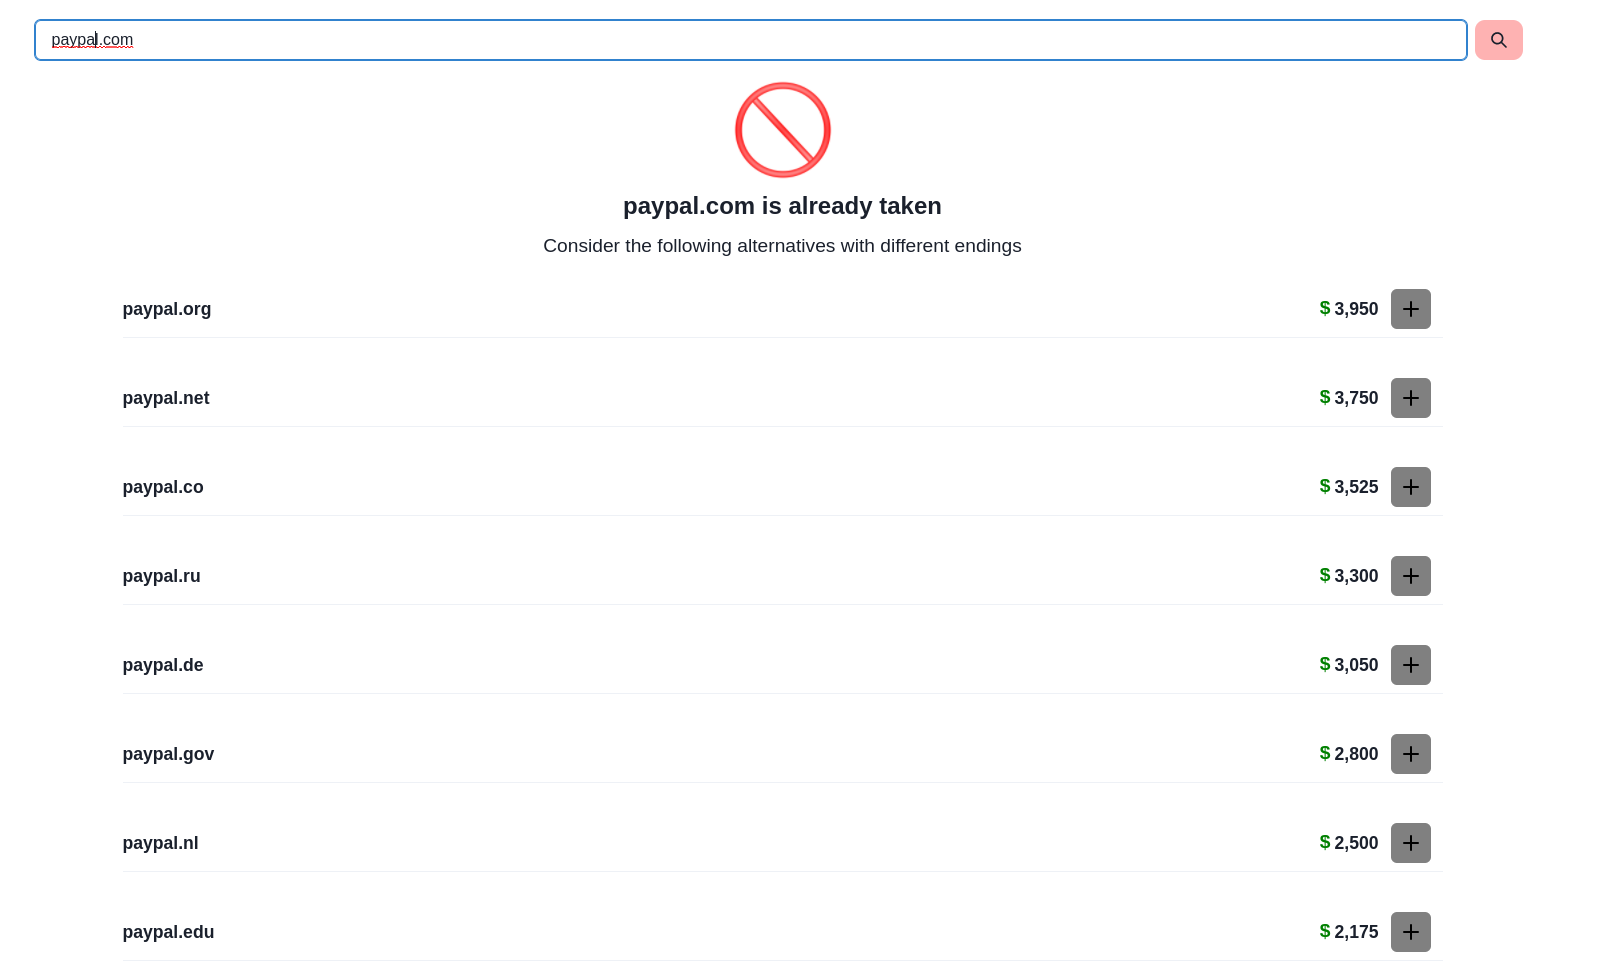
\includegraphics[width=0.8\textwidth]{figures/section2/marketplace_unavailable.png}
    }
    \hfill
    \subfloat[Marketplace available\label{subfig:marketplace-available}]{%
        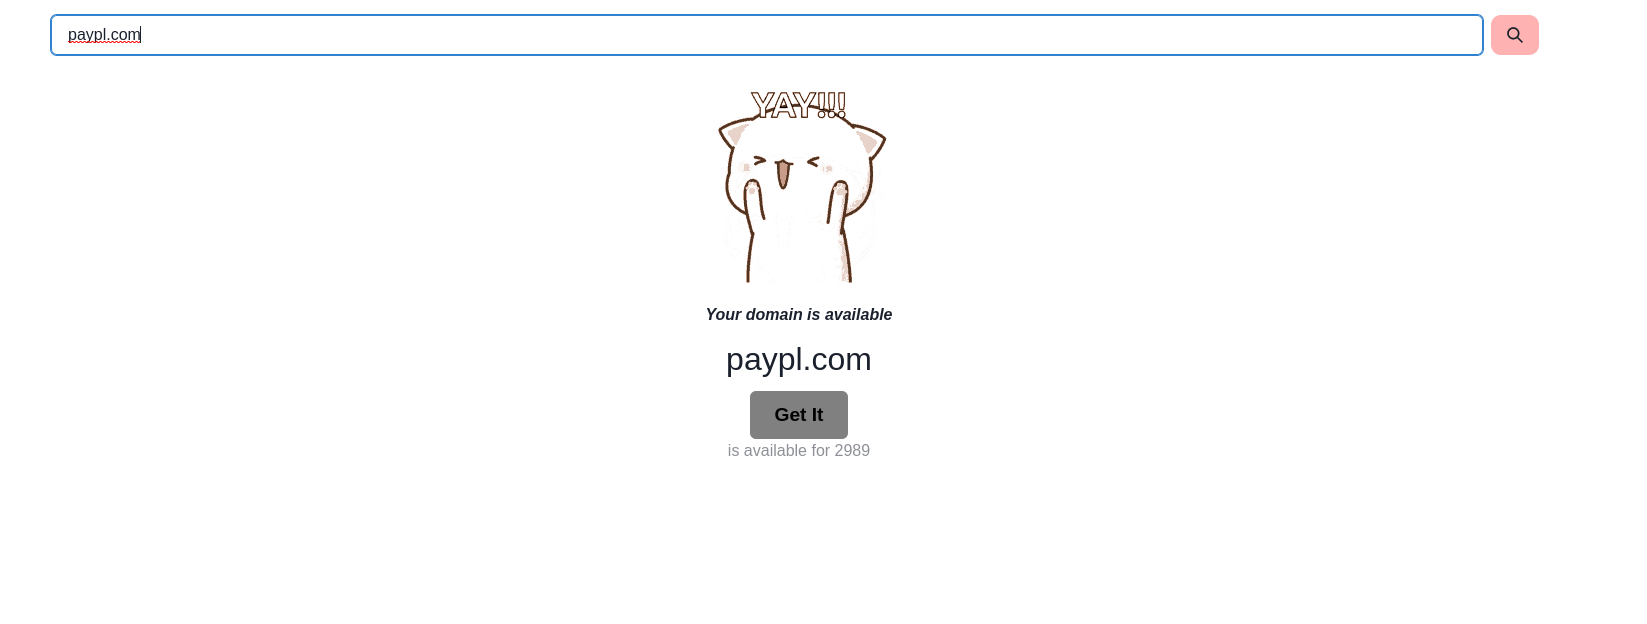
\includegraphics[width=0.45\textwidth]{figures/section2/marketplace_available.png}
    }
    \hfill
    \subfloat[Marketplace invalid\label{subfig:marketplace-invalid}]{%
        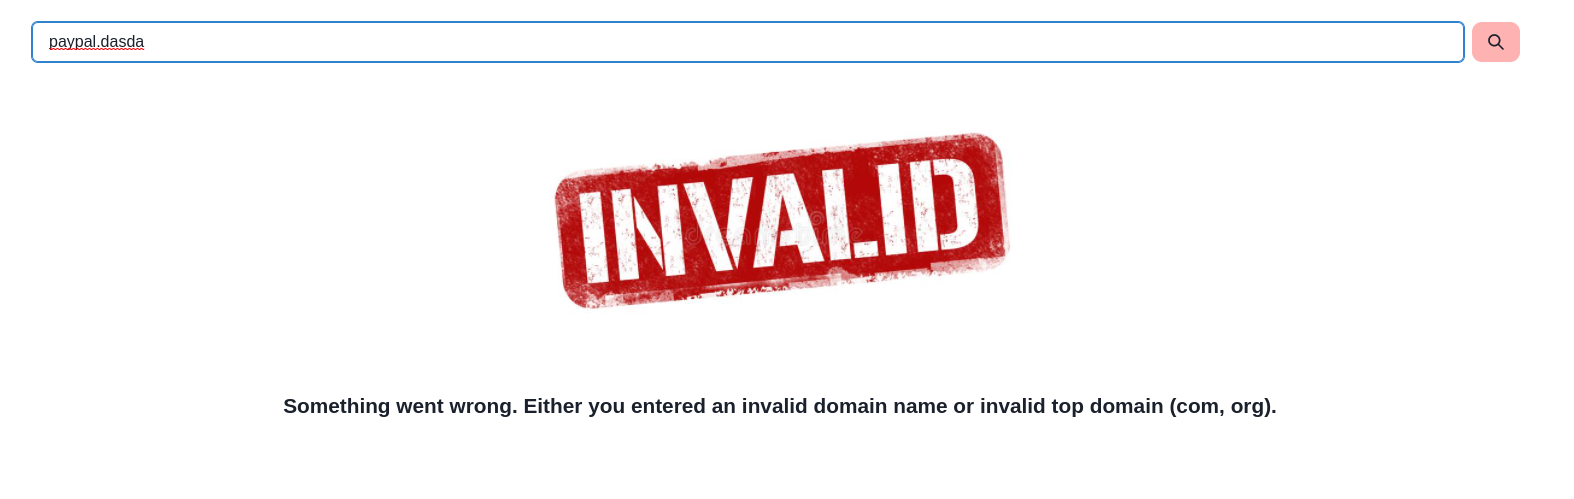
\includegraphics[width=0.45\textwidth]{figures/section2/marketplace_invalid.png}
    }

    \label{fig:marketplace-state}
    \caption{Different stages of the marketplace}
\end{figure}

The initial formula to calculate the cost was based on trial and error. Although not an actual scale, we set the cost to show that domains closer to real-world domains will have a higher cost. We later scaled the cost to adjust the game's difficulty.

\subsubsection{Emails}
The emails component ties up the game by generating and sending emails based on attacker skills and the current domain. The system randomly chooses an email from 30 available emails based on the user input (active and passive skills). These emails were handpicked to replicate real-life phishing attempts and include the most commonly found phishing emails. As a result, emails in the system include common phishing emails and tricks used by attackers such as log-in, welcome emails, limited account emails, etc.


Before discussing sending email and efficiency, let us discuss how each skill impacts the email generation process. As mentioned in the attacker component section, passive skill does not require additional input from the player and improves the generated email after training them. Spelling, grammar, and styling in our game fall under passive skills. Before players train on spelling and grammar, they will be required to recognize spelling and grammar errors. We wanted to point out spelling and grammar errors as they are commonly found in poorly worded phishing emails and recognized as one of the common ways to differentiate phishing emails with legitimate errors. Since we do not want the user to spend all their time finding language errors, we generate emails with proper grammar and spelling after training.

Similarly, styling increase the visual appealingness of the email with the help of images, header, footer, and better-styled emails. Emails sent by an organization generally contain images and styling. Attackers use this fact and try to trick victims by including company logos and images.

\begin{figure}[ht]
    \centering

    \subfloat[Emails generated after training on passive skills generate emails with proper grammar and spelling with styling\label{subfig:passive-trained}]{%
        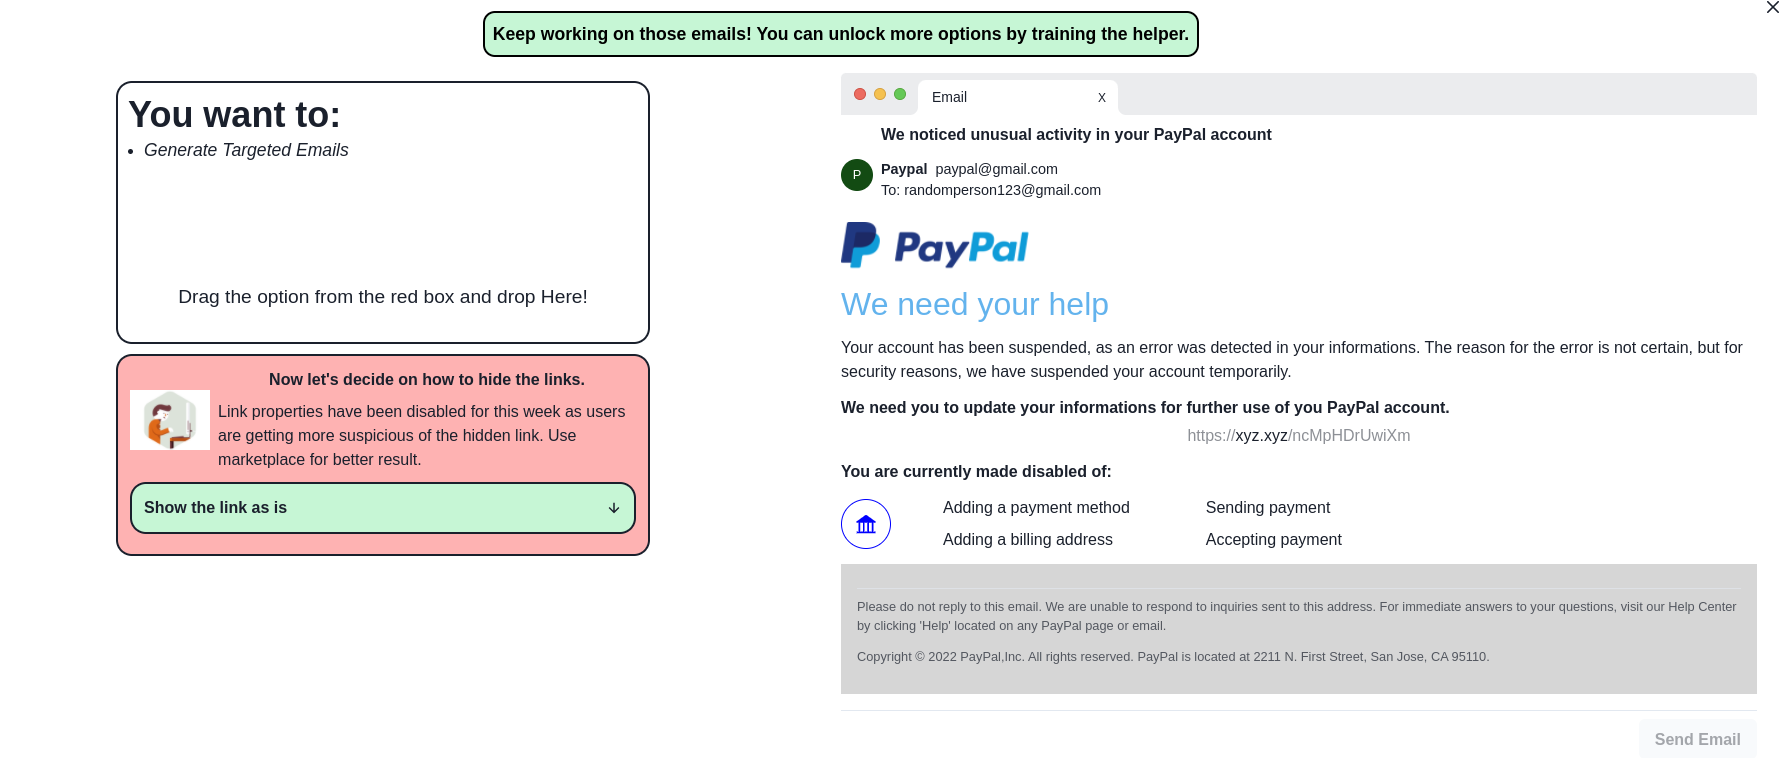
\includegraphics[width=0.75\textwidth]{figures/section2/passive_trained.png}
    }
    \hfill
    \subfloat[Emails generated before training on passive skills contains spelling and grammar error with no styling (contains text only)\label{subfig:passive-untrained}]{%
        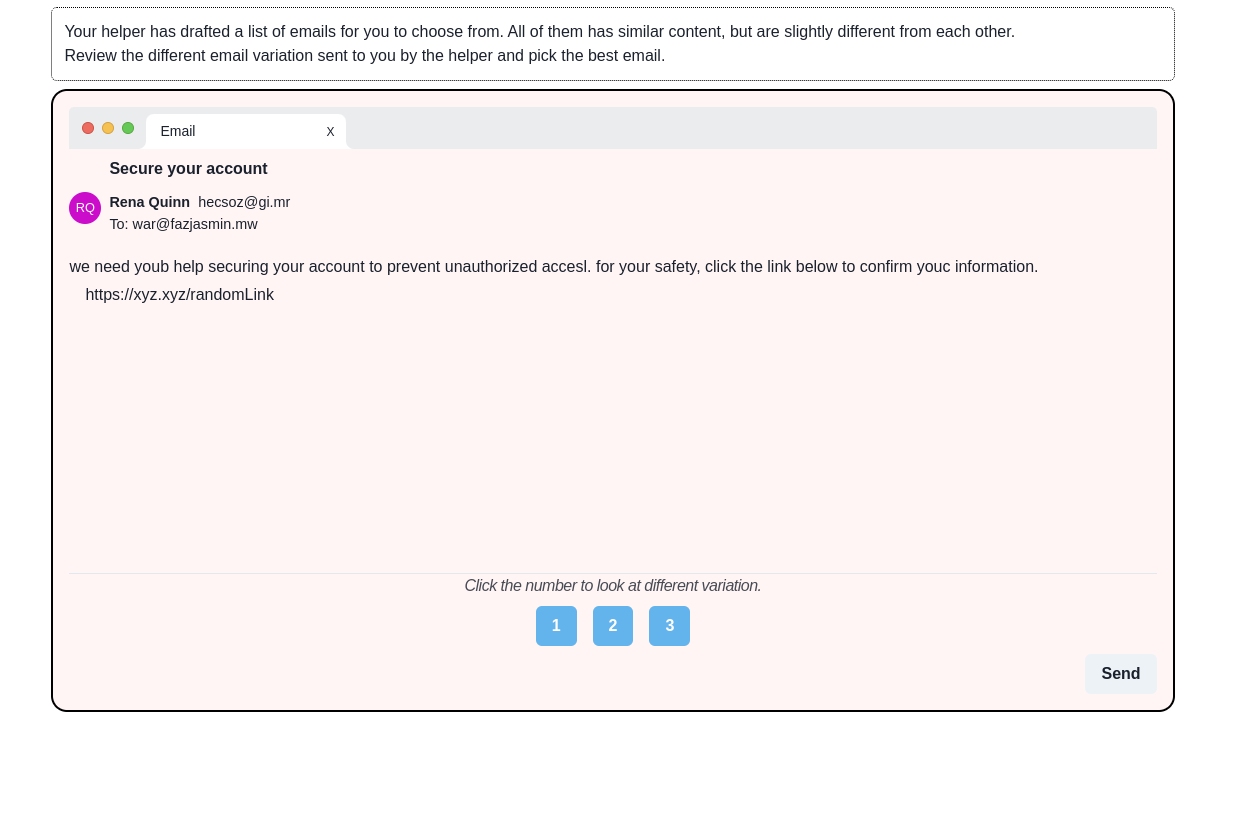
\includegraphics[width=0.75\textwidth]{figures/section2/passive_untrained.png}
    }
    \hfill

    \label{fig:passive}
    \caption{Emails generated after training vs before training on passive skills}
\end{figure}

Active skills give the user more options while generating emails. Our game's active skills are links, research, and spoofing. Each of these options allows the user to modify the generated email. We discuss each of these skills in detail below.

Research skill allows the player to generate targeted emails or generic emails. Our game approaches the concept of spear-phishing with targeted email. Before training on research, all the generated emails will be generic, and players do not get an option to send targeted emails. Generic emails do not contain any specific user information, whereas targeted email contains some form of user-specific information such as an address and name.

\begin{figure}[ht]
    \centering
    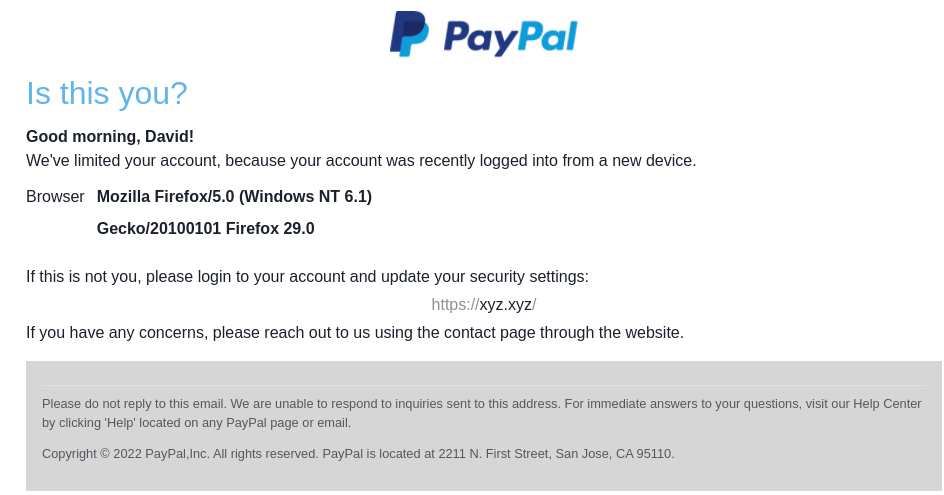
\includegraphics[width=0.9\textwidth]{section2/targeted.png}
    \caption{Example of a targeted email generated by the system}
\end{figure}

Both targeted and generic emails are pre-defined in the system. The system filters out targeted/generic emails and randomly chooses an email from the remaining emails based on the user input.

Our links skill attempts to cover URL/link training many current phishing training games cover. Training helper on link unlocks different ways to hide the link when generating an email. These options were chosen based on real-world phishing emails. The game includes four different ways to hide the link:

\begin{enumerate}
    \item \textbf{Hide under button or text}\\
          One common phishing trick is to hide the actual link behind some text or button. We replicate this behavior with our "Hide link" option, which displays either some text or button but redirects to another destination. To familiarize users with different text and buttons, we randomly hide the text either behind the button (Example figure \ref{fig:hide-button}) or a randomly chosen text (Example figure \ref{fig:hide-text}). Then, players can hover over the text or button to visualize the link (similar to real email clients). Since we did not want the text or button to look the same every time the option was chosen, we randomly selected pre-determined texts and links such as "Go to PayPal," "Click here," "www.paypal.com/help," and similar alternatives.

          \begin{figure}[ht]
              \subfloat[The actual link is hidden behind the button]{%
                  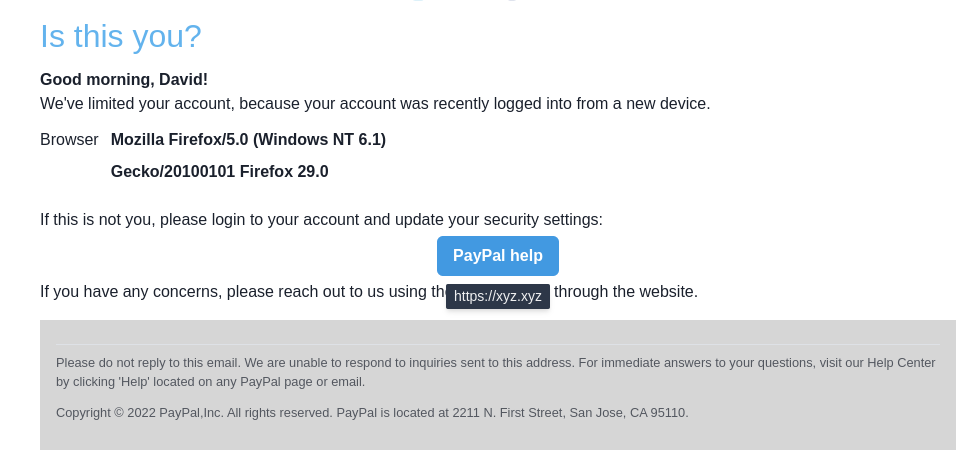
\includegraphics[width=0.48\textwidth]{figures/section2/hide_button.png}
                  \label{fig:hide-button}
              }
              \hfill
              \subfloat[The actual link is hidden behind the text]{%
                  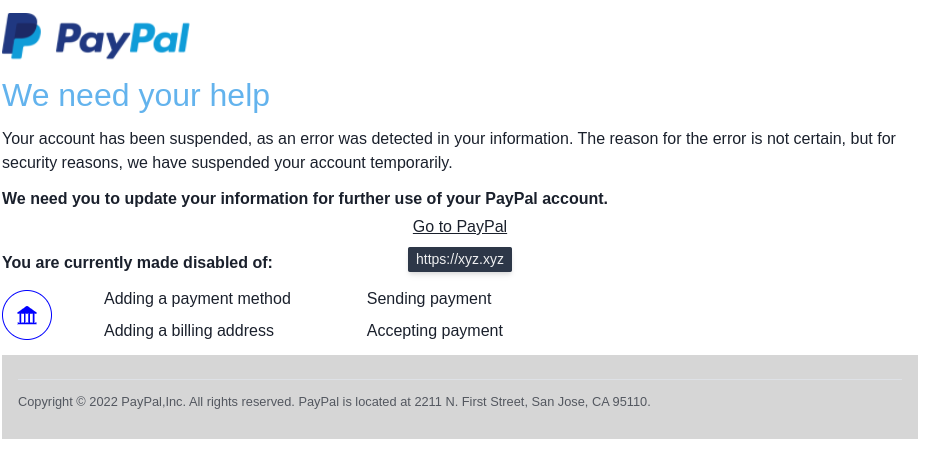
\includegraphics[width=0.48\textwidth]{figures/section2/hide_text.png}
                  \label{fig:hide-text}
              }
              \caption{Examples of hiding the actual link behind text or button}
          \end{figure}

          The primary goal of this option is to train the user to not trust the displayed link or text and be careful about clicking on the link.

    \item \textbf{Link shortner}\\
          During our survey of phishing emails, we noticed attackers use URL shorteners to confuse the end-users. A URL shortener is a tool that creates a short, unique URL that will redirect to the specific website of the user choosing. There are multiple free URL shortening services that shorten the URL with a button click. TinyURL, Bitly, Short.io, BL.INK are some popular examples of shortening services. Table \ref{tab:shortner} shows an example of a different URL shortener. The shortened links do not expose the actual domain it redirects to. Phishers use this fact by hiding the actual domain with the help of shortening services.

          \begin{table}
              \centering
              \begin{tabular}{c p{0.7\textwidth}}
                  \textbf{Service} & \textbf{Shortner}                                                                               \\
                  \hline
                  URL              & https://www.uno.edu/academics/colaehd/ehd/elcf/educational-leadership-graduate-programs/masters \\
                  \hfill
                  TinyURL          & https://tinyurl.com/5n6ehd6k                                                                    \\
                  bitly            & https://bit.ly/3CGFfBC                                                                          \\
                  is.gd            & https://is.gd/MKZdLO                                                                            \\
                  Tiny             & http://tiny.cc/unjpuz                                                                           \\
                  RB.GY            & https://rb.gy/nrwbqb                                                                            \\
              \end{tabular}
              \caption{Example of different URL shortner }
              \label{tab:shortner}
          \end{table}

          \begin{figure}[h!]
              \centering
              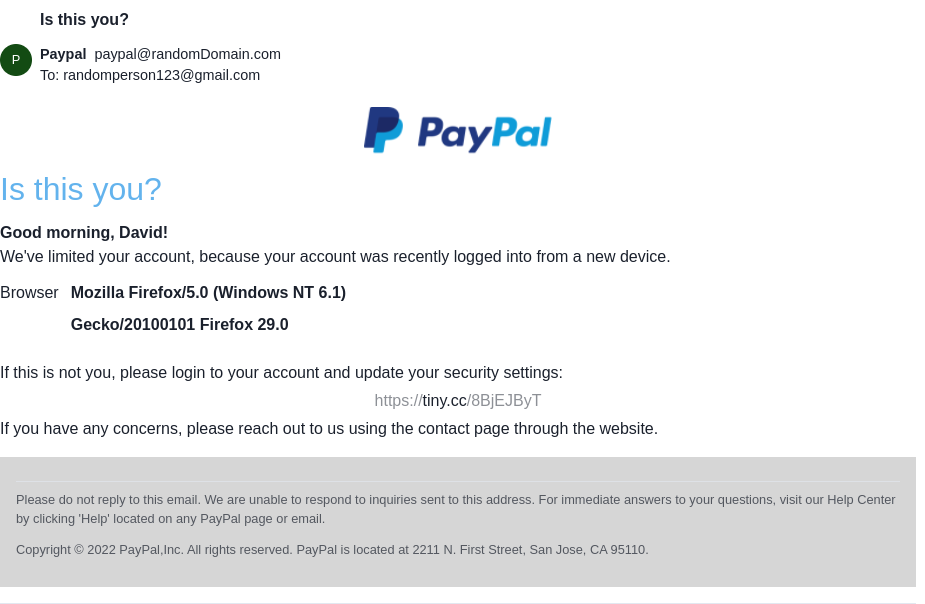
\includegraphics[width=0.9\textwidth]{figures/section2/shortener.png}
              \caption{Example of a URL shortner}
              \label{fig:shortner}
          \end{figure}

          Figure \ref{fig:shortner} shows an example of email generated with shortner option. The primary goal of this option is to familiarize players with different URL shortening services and how they can be used to hide actual links. In addition, we want the user to know about multiple shortening services. Hence, every time the user chooses to hide the link with the shortening service,  we randomly choose one of the shortening services and attach a nano id. Table \ref{tab:shortner} shows different links included in the game.

    \item \textit{Confusion}\\
          The confusion option tries to train users to recognize legit-looking domains. We focus on subdomains for this option as subdomains are free and can be anything (including existing organization names). Phishing links attempt to confuse the users by including the organization name as a subdomain. For example, "paypal.xyz.com" may look like a PayPal domain but is a page in xyz.com.

          \begin{figure}[ht]
              \centering
              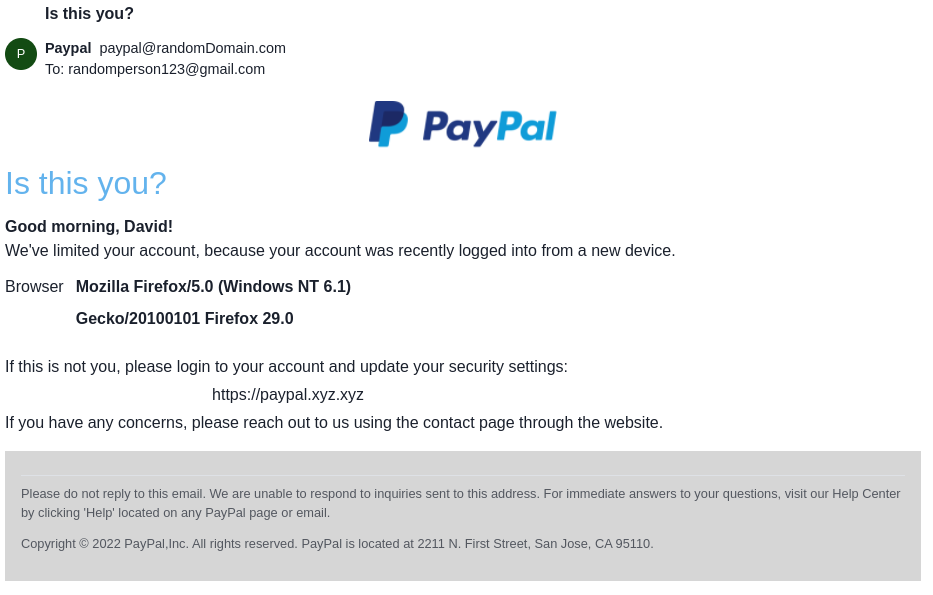
\includegraphics[width=0.9\textwidth]{figures/section2/confusion.png}
              \caption{Example of a email generated with link confusion}
              \label{fig:confusion}
          \end{figure}

    \item \textit{Display link as is}\\
          The display link as is option allows the user to see the actual link without any modification. This option is useful when the domain purchased by the player is very similar to PayPal. For example, "paypai.com" (with an i) looks similar enough to paypal.com. This can easily trick the users into clicking the link if they are not paying attention. We use this option to train users on a similar-looking domain bought from the marketplace.

\end{enumerate}


Player select the link hiding method with an interactive drag and drop approach. One of the primary goals of link hiding techniques was to teach the player how each option changes the emails. Therefore, our gameplay immediately visualizes the player's changes to the generated email. This allows the players to see how the links can be used in context to the email.

The final active skill in the game is spoofing. Existing games do not focus on training users on spoofing. However, users can easily get tricked into giving sensitive information if they receive emails from a familiar source. Various free services (Example: figure \ref{fig:spoof_sender}) send emails with custom header (custom to, reply-to, subject fields in the email) without additional verification.

\begin{figure}[ht]
    \centering
    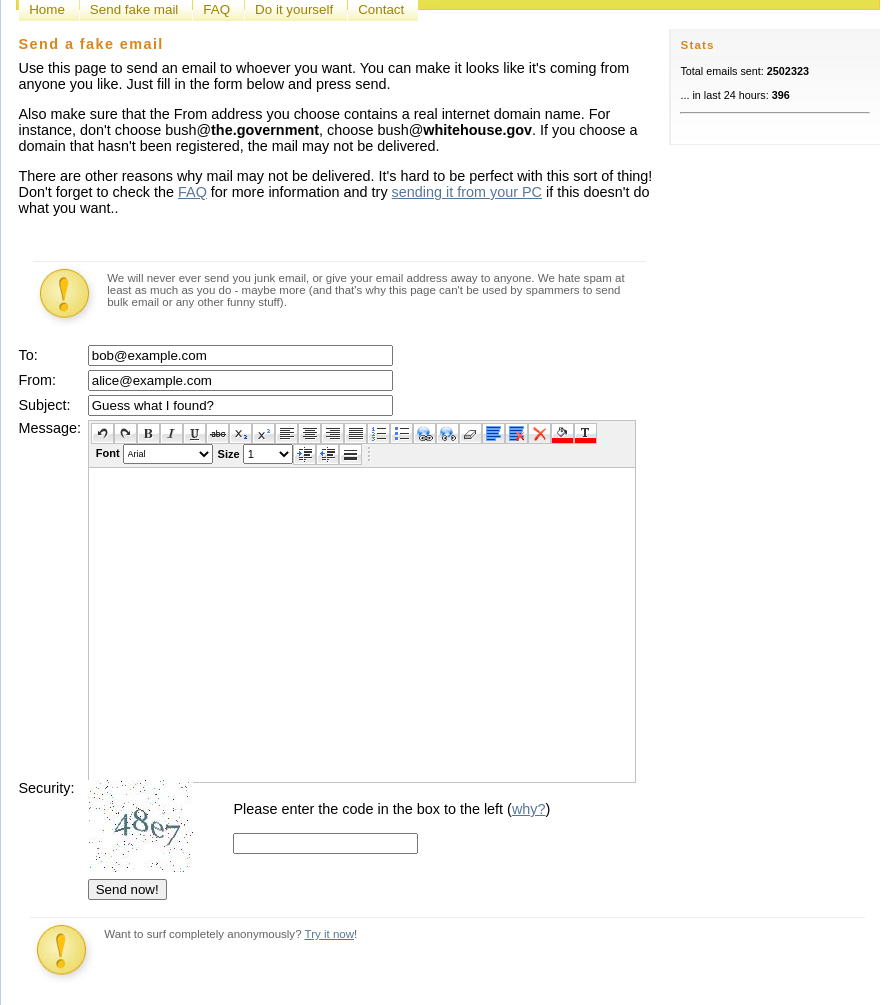
\includegraphics[width=0.4\textwidth]{figures/section2/spoof_sender.png}
    \caption[Fake email sender]{Example of a fake email sender. User can send the email to any email address as any sender.}
    \label{fig:spoof_sender}
\end{figure}

After the player unlocks the "spoof" skill, we allow the player to change the email address of the sender to any valid email address. The primary goal is to show the user that the sender can be any one and user have to pay attention to other details of the emails too.

\begin{figure}[ht]
    \centering
    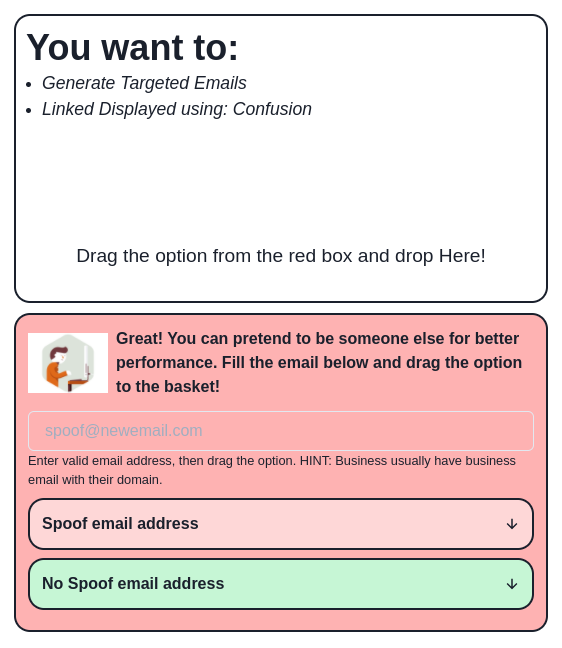
\includegraphics[width=0.4\textwidth]{figures/section2/spoofing.png}
    \caption{Spoofing option in game}
    \label{fig:spoofing}
\end{figure}

\subsection{Email efficiency}
The efficiency of the email generated by the system depends on the options chosen by the user. Each skill improves the efficiency of the email. The efficiency of the email is calculated as

\begin{center}[ht]
    \resizebox{\textwidth}{!}{
        \begin{math}
            E= \frac{\text{Sum of trained passive skill points + Sum of skill point of active skills chosen by the user}}{\text{Total Available skill points}} \times 100\%
        \end{math}
    }
\end{center}


Table \ref*{tab:efficiency} shows the max efficiency point for each skill in the game. The efficiency of passive skills is either 0 (if absent) or max efficiency points (if present), whereas active skills efficiency is calculated based on user input. Generating targeted (spear phishing) is more efficient as it contains personal information in the emails. To replicate this, we add 20 points to the efficiency if the generated email is targeted.

\begin{table}[ht]
    \centering
    \begin{tabular}{l c}
        Skill    & Max Efficiency Point \\
        \hline
        Spelling & 5                    \\
        Grammar  & 5                    \\
        Styling  & 10                   \\
        Research & 20                   \\
        Links    & 25                   \\
        Spoofing & 25                   \\
    \end{tabular}%
    \caption{Efficiency of each option}
    \label{tab:efficiency}
\end{table}

Different link hiding skill have different efficiency although really close to each other. Hiding the link behind the text gives 18 points, shortening the link gives 20 points and using confusion gives 25 points. When the player decides to display link as is, we calcualte the string similarity of the user domain with "paypal.com". If the similarity is greater than 80\%, we add 20 points to the efficiency else we add 3 points to efficiency.

We want to encourage users to notice that they can pretend to send the email as anyone. We comapre the domain in the email chosen by the user with "paypal.com". We assign variable points to the efficiency based on the similarity.

\begin{table}[h!]
    \centering
    \begin{tabular}{l c}
        Similarity & Point \\
        \hline
        90\%       & 20    \\
        80\%       & 18    \\
        60\%       & 7     \\
        Below 60\% & 0     \\
    \end{tabular}%
    \caption{Similarity of spoofed email domain and points assigned}
    \label{tab:similarity_spoofed}
\end{table}

We considered different keywords used in real emails. If the name included keywords "contact", "help","info","no-reply" or "noreply", we add 5 points to the efficiency. Similarly, if the email contains "paypal" in the name, we add 10 points.

'\subsection{Previous Iteration}
Initially, the game was an open system, where users could train with any skill at any given point (given they had enough amount to train). We used time to incentivize users to explore different options and generate efficient emails. The game had the same goals, options, and components but required players to watch the time.

\begin{figure}[ht]
    \centering
    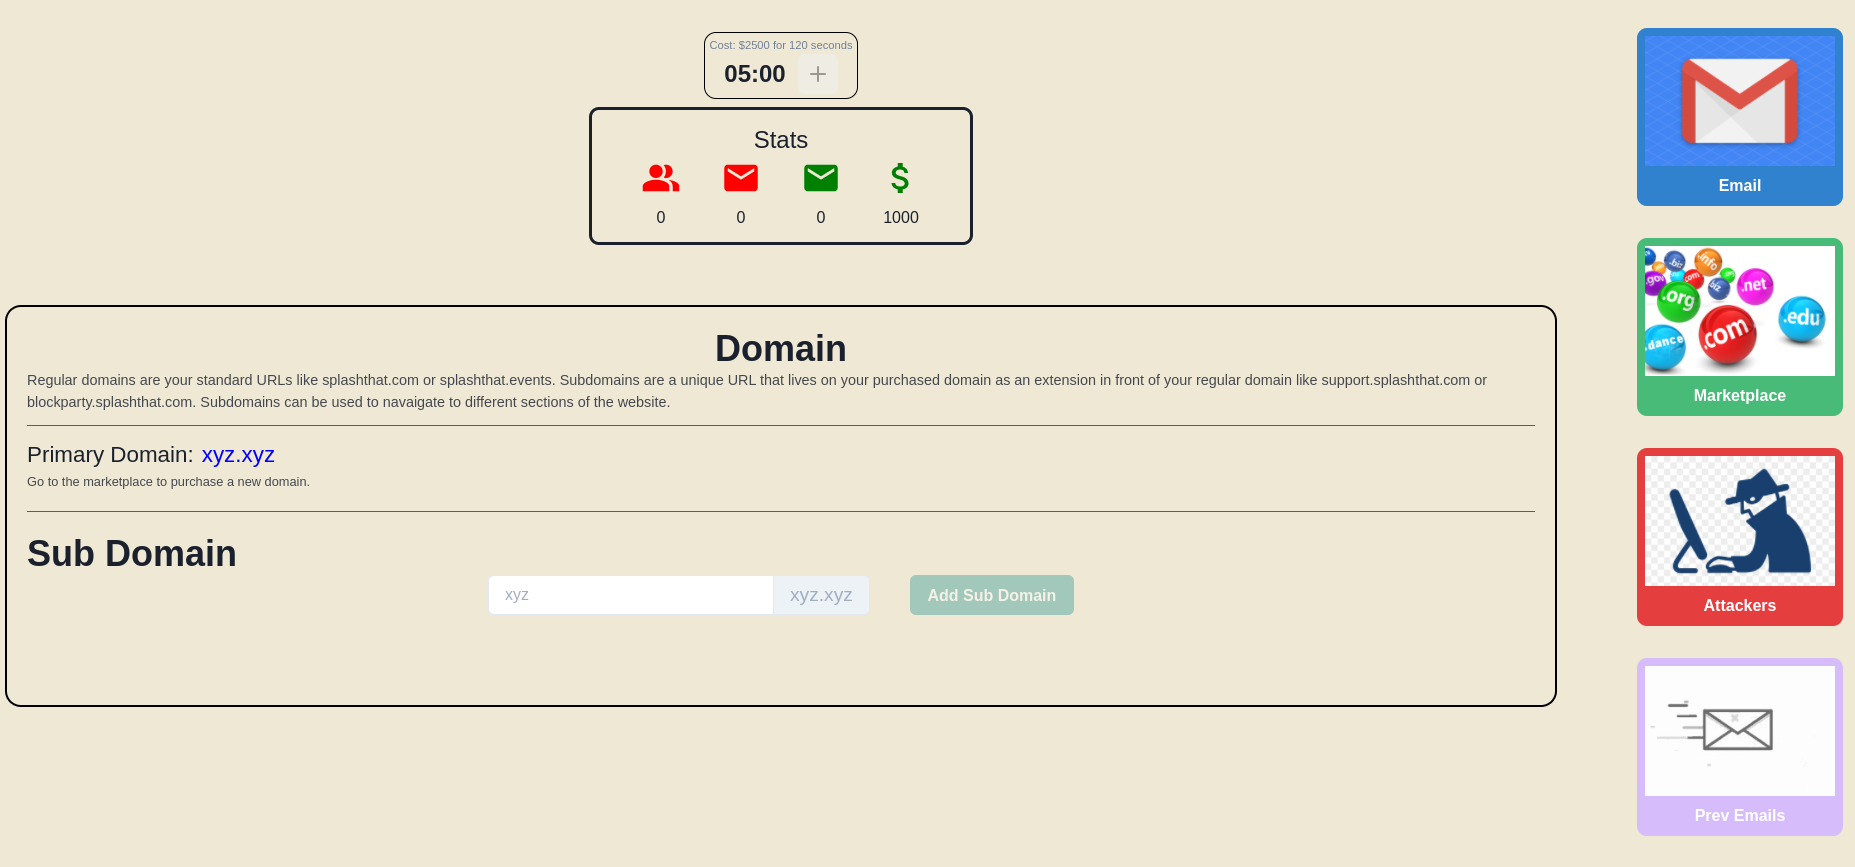
\includegraphics[width=0.9\textwidth]{figures/section2/game_initial.png}
    \caption[Initial version of the game]{Initial version of the game included timer to incentivize the user to complete the game.}
\end{figure}

We noticed a few drawbacks in the initial testing of the game. First, we realized that players were worried about running out of time and were not reading all the emails and options. This challenged us to balance the game such that users had enough time to read all the emails but could not brute force (send unlimited emails to achieve the goal) through it. However, different players played the game at different paces, which made us realize that time might not be the best way to incentivize the players to finish the game.

Second, we wanted to ensure that all the players had a similar experience and explored all possible training options. Unfortunately, the open system prevented us from ensuring all the players explored the training module in the same order. It also allowed the player to train on multiple modules simultaneously because of which players might not learn all the objectives of each option.

We developed a new design to mitigate these challenges that ensured players focused on each training module. Our current design locks the training skills and forces users to use specific training skills each week.

\subsection{Weekly Goals}
The game's current design divides the game into four parts (week). Each week unlocks new skills that the user must train on to reach the goal. Table \ref{tab:weekly-goals} shows what skills are unlocked each week and the skills we want the user to focus on. The weekly goals are adjusted based on the efficiency of the emails for the current week. As discussed above, the user's current skills determine the efficiency of the email.

\begin{table}[ht]
    \centering
    \resizebox{\textwidth}{!}{%
        \begin{tabular}{|c|l|l|c|}
            \hline

            \textbf{Week} & \textbf{Trainable Skills}      & \textbf{Skill focus}       & \textbf{Weekly Goal} \\
            \hline
            1             & None                           & Spelling, Grammar          & 5000                 \\
            2             & Spelling, Grammar, Links       & Links                      & 5000                 \\
            3             & Marketplace, Styling, Research & Spear phishing and domains & 5000                 \\
            4             & Spoofing                       & Spoofed emails             & 5000                 \\
            \hline
        \end{tabular}%
    }
    \caption{Weekly goals}
    \label{tab:weekly-goals}
\end{table}

Week 1 does not contain any trainable skill and solely focuses on language in the email. We want the player to know that low-tier phishing emails may contain spelling or grammar problems, whereas official emails are usually proofread and do not contain these issues.

Week 2 lets the user train on spelling, grammar, and links. Players can remove spelling and grammar errors by training language skills and entirely focus on different link hiding techniques.

Week 3 opens the marketplace along with styling and research. At this point, users have explored different ways to hide the link, and we want to focus on links that might look similar to trick the user. To force users to explore different domains, we disable all link hiding techniques and force users to show the link. We want users to pay close attention to the link they are clicking.

Week 4 disables the marketplace and unlocks spoofing. We let the user hide the link and let them be anyone they want.